% Anthology of Computers and the Humanities (CHR) submission.
% Add the 'final' option to documentclass for the camera-ready version.
\documentclass{anthology-ch}

\usepackage{booktabs}
\usepackage{graphicx}
\usepackage{iftex}
% Polytonic Greek: render inline Greek words in a font with full coverage.
\ifXeTeX
  \newfontfamily\greekfont[
    Path=fonts/Noto_Serif/static/,
    Extension=.ttf,
    UprightFont=NotoSerif-Regular,
    BoldFont=NotoSerif-Bold,
    ItalicFont=NotoSerif-Italic
  ]{NotoSerif}
  \newcommand{\gk}[1]{{\greekfont #1}}
\else
  \newcommand{\gk}[1]{#1}
\fi

\title{Knowing When the Author Is Absent: Interpretable, Calibrated, Open-Set Authorship Verification for the Pseudo-Chrysostoms}

% TODO: replace with real author name(s), ORCID, and affiliation before submission.
\author[1]{First Author}[
  orcid=
]

\affiliation{1}{Department, University, City, Country}

\keywords[eng]{authorship verification, open-set verification, conformal prediction, stylometry, patristics, pseudo-Chrysostomica, Severian of Gabala, Ancient Greek}

\pubyear{2026}
\pubvolume{1}
\pagestart{1}
\pageend{1}
\paperorder{1}
\conferencename{Proceedings of the Computational Humanities Research Conference}
\conferenceeditors{}
\doi{00000/00000}
\customhead{}

\addbibresource{bibliography.bib}

\begin{document}

\maketitle

\begin{abstract}
More than fifty homilies of Severian of Gabala survive in Greek only because scribes copied them under the name of his rival, John Chrysostom; recovering such attributions is a long-running task of patristic philology, and one already addressed with a neural verifier. We revisit it not to attribute the texts afresh but to make each verdict auditable and to give the verifier something no prior system for this material has: the ability to say, with a guarantee, that the author is not among the candidates. Building entirely on openly licensed Greek corpora and on hand-crafted features -- function words, part-of-speech trigrams, and character affixes -- we wrap a Bootstrap Distance Impostors verifier in a conformal layer that turns each score into a prediction set with distribution-free coverage and a principled reject option. On held-out reference authors the $90\%$ set contains the true author $90\%$ of the time; when the author is absent from the candidate set the verifier abstains $88$--$96\%$ of the time. Two further controls keep the verdicts honest: a provenance control that stops shared digitization from masquerading as shared authorship, and a per-channel decomposition that reports which linguistic evidence drives each judgement. Applied to twenty-two groups of pseudo-Chrysostomica, the calibrated verifier recovers the published attribution for every ground-truth group whose author is a candidate -- three of three, including the one genuinely Chrysostomic group -- while a nearest-author baseline misattributes them all to Severian. Neither a retrained Siamese metric nor a frozen contextual encoder, added as extra channels, improves on the transparent features or overturns their verdicts: here legibility costs no accuracy.
\end{abstract}

\section{Introduction}

The corpus transmitted under the name of John Chrysostom accreted, over late antiquity and the Byzantine centuries, a large body of homilies he did not write. Many are simply anonymous; a substantial number belong to identifiable contemporaries whose works travelled more safely under a celebrated name. The clearest case is Severian of Gabala, Chrysostom's rival at the Synod of the Oak: almost all of his Greek homilies survive only among the Chrysostomic spuria printed in \emph{Patrologia Graeca} 48--64, and his genuine works occupy \textsc{cpg} 4185--4295 \cite{cpg,severian_wiki}. Sorting the pseudo-Chrysostomica -- assigning each item to Severian, to another named author, or to no one in particular -- has occupied philologists since de Aldama's \emph{Repertorium} \cite{dealdama1965} and, above all, the sustained work of Sever Voicu \cite{voicu}.

Computational stylometry offers one route into this material. \textcite{clerice2023} verified a set of pseudo-Chrysostoms with a Siamese network trained on function words, part-of-speech trigrams, and character affixes. More recent work has turned to large language models and fine-tuned encoders: \textcite{gorovaia2024} evaluate GPT-4o and comparable systems on Latin patristic verification, and \textcite{schmidt2024} fine-tune Greek pre-trained models for the authorship of the pseudo-Dionysian \emph{Ars Rhetorica}. These approaches are powerful, yet their authors note a shared limitation for philological use: the models are steered with difficulty, are ``easily misled by semantics,'' and do not readily explain a verdict \cite{gorovaia2024}. For a scholar weighing an attribution, an unexplained judgement is of limited evidential value. Closest to the present study, \textcite{clerice2025} verify authorship across a massively anonymous Old French tradition with a feature-based imposters method; we adopt the same family of technique and press on its explanatory potential for Greek.

Our study stands closest to \textcite{clerice2023}, and it is worth marking the overlap plainly. That work targets the same corpus, represents each text with the same three channels -- most frequent words, character affixes, and part-of-speech trigrams -- trains a Siamese network with a signal-to-noise-ratio distance (AUC-ROC $0.845$), and grades its verdicts against Voicu's twenty-one groupings. We reuse those features and, as a cross-check, a reproduced network of the same kind; what we add is the apparatus that makes a verification claim auditable. The central addition is a conformal reject option that equips the verifier with a distribution-free guarantee and, for the first time on this material, a principled abstention when the author is absent from the candidate set. Around it sit three further differences: the reference is rebuilt entirely from openly licensed corpora, so the pipeline can be re-run; a provenance control separates authorship from the shared digitization of the sources; and a per-channel decomposition, with a table of the words that most distinguish the rival authors, exposes the linguistic basis of every judgement. The neural verifier of \textcite{clerice2023} is a corroborating instrument here, not the method under test.

This paper pursues the complementary path. We keep the interpretable, feature-based method, reproduce it on openly licensed data so the results can be checked and reused, and add the apparatus a verification claim requires. Our contributions are: (1) a reproduction of the feature pipeline of \textcite{clerice2023} on open corpora; (2) the central contribution, an \emph{open-set} conformal verification protocol -- Bootstrap Distance Impostors \cite{nagy2024} wrapped in a conformal layer \cite{vovk2005,angelopoulos2023} that gives every verdict distribution-free coverage and a validated reject option, so the method can abstain, with a guarantee, when the true author is not among the candidates; (3) two auditing controls around it -- a provenance control that keeps shared digitization from being read as shared authorship, and a per-channel decomposition of the evidence; and (4) an evaluation against the published \textsc{cpg} attributions, on which the method recovers the true author for every ground-truth group whose author is a candidate and, for the anonymous majority, supplies confidence-graded, inspectable proposals. Two neural cross-checks -- a retrained Siamese metric and a frozen contextual encoder used as an extra channel -- match the transparent features without beating them, evidence that the interpretable representation sacrifices no accuracy.

\section{Data}

\paragraph{Reference corpus.} We assemble a reference of clean, critically edited Greek from two open sources: the Open Greek and Latin \emph{First1KGreek} project \cite{first1k} and the Patristic Text Archive \cite{pta}. After repairing author labels and balancing the corpus so that no writer dominates (each author capped at 30 works, singletons removed), the reference holds 1{,}082 works by 113 authors. The candidate patristic authors include Severian of Gabala and John Chrysostom, together with Eusebius, Cyril of Alexandria, Theodoret, Athanasius, and Origen; Severian is represented by the critically edited \emph{Homiliae Pseudo-Chrysostomicae} \cite{hpc}.

\paragraph{The pseudo-Chrysostoms.} The texts under study are 69 homilies grouped into 22 sets (PC1--PC21), all transmitted under Chrysostom (\textsc{tlg} author 2062) and printed in \emph{PG} 48--64; the Thesaurus Linguae Graecae marks all but one as spurious. Each group corresponds to a work or cluster of works with a Migne reference and, where known, a \textsc{cpg} number.

\paragraph{Features.} Following \textcite{clerice2023}, each text is represented by three channels: the 1{,}000 most frequent function words (FW), the 100 most frequent part-of-speech trigrams (POS), and the 1{,}000 most frequent character affix trigrams (AFF). Part-of-speech tags are produced by a Greek BERT tagger \cite{superpeitho}. Because part-of-speech features are only comparable when produced by the same tagger, we exclude from this study a set of optical-character-recognition texts (from \emph{Patrologia Graeca} scans \cite{pgcorpus}) whose supplied tags follow a different scheme; the pseudo-Chrysostoms and all patristic candidates are tagged uniformly.

\section{Method}

\paragraph{Feature-space distances.} Within each channel we standardise features across the reference (a Burrows-style $z$-transform \cite{burrows2002}) and represent each author by the centroid of their works. A text's distance to a candidate is the mean absolute $z$-difference to that centroid, averaged over channels. Nearest-centroid attribution serves as a baseline.

\paragraph{Calibrated verification.} Nearest-centroid answers ``which candidate is closest,'' not ``is this text by author $A$.'' For the latter we use an impostors-based verifier of the General Impostors \cite{koppel2014,kestemont2016} and Bootstrap Distance Impostors \cite{nagy2024} family -- the technique \textcite{clerice2025} apply to a comparable anonymous tradition: to score a text $q$ against author $A$, we repeatedly draw a random half of the features and a random pool of impostor documents, and record how often $q$'s nearest $A$-document is closer than its nearest impostor. The score is the fraction of iterations $A$ wins. To keep the comparison fair when authors differ greatly in size -- Severian has far more attributed works than Chrysostom -- we subsample a fixed number of target documents per iteration. Following \textcite{nagy2024} we read this score as a statistical likelihood and attach a 95\% bootstrap confidence interval to it.

\paragraph{Provenance control.} Because the pseudo-Chrysostoms and the Severian comparanda are edited within the same project, a similarity could reflect shared digitization rather than authorship. Since no second edition of Severian exists in our data, we control for this within the Patristic Text Archive: if a group prefers Severian over \emph{other} same-provenance authors (Eusebius, Cyril, Athanasius, Theodoret), the signal is not merely editorial.

\paragraph{Per-channel decomposition.} Finally we run the verifier on each channel separately. A verdict supported by function words, part-of-speech trigrams, and affixes alike is more trustworthy than one carried by a single channel; affixes in particular track orthography and are the most sensitive to editorial convention.

\paragraph{Conformal reject option.} The impostors score is a point estimate. To attach a guarantee to it, and to let the verifier decline when no candidate fits, we wrap it in split-conformal prediction \cite{vovk2005,angelopoulos2023}. Treating the reference candidates as the closed set of possibilities, we take $1-\mathrm{BDI}(q,A)$ as a nonconformity score and calibrate its same-author distribution on the reference. This turns the score into a conformal $p$-value for each candidate and, at a level $\alpha$, a prediction \emph{set}: the candidates whose $p$-value exceeds $\alpha$. A singleton is a confident attribution, several candidates an unresolved one, and an empty set a principled abstention -- the signal that the true author is probably not among the candidates. By construction the set has distribution-free coverage: when the author is a candidate, the true author lies in the $1-\alpha$ set at least a $1-\alpha$ fraction of the time.

\section{Results}

\subsection{The verifier works, and three methods agree}

Before applying the verifier to disputed texts, we measure it on labelled reference authors. From authors with at least five works we build 630 same/different-author verification problems and score each with three independent feature-space methods: the impostors win-fraction used here, Burrows's Delta to an author centroid, and cosine similarity. All three separate the classes well (Table~\ref{tab:benchmark}, Figure~\ref{fig:roc}); the impostors method is the most accurate (ROC-AUC $0.998$, $F_1$ $0.957$), and the three scores agree closely (Spearman $\rho$ between $0.81$ and $0.95$). The verdicts that follow are therefore both accurate and robust to the choice of scorer.

\begin{table}[t]
  \centering
  \small
  \begin{tabular}{lccccc}
\toprule
Method & ROC-AUC & AP & Prec. & Rec. & F1 \\
\midrule
Impostors (this paper) & 0.961 & 0.945 & 0.918 & 0.867 & 0.891 \\
Burrows's Delta & 0.938 & 0.914 & 0.833 & 0.833 & 0.833 \\
Cosine & 0.959 & 0.927 & 0.859 & 0.878 & 0.868 \\
\bottomrule
\end{tabular}

  \caption{Verification benchmark on 630 problems from the reference authors. The impostors method used in this paper is the most accurate, and Delta and cosine corroborate it.}
  \label{tab:benchmark}
\end{table}

\begin{figure}[t]
  \centering
  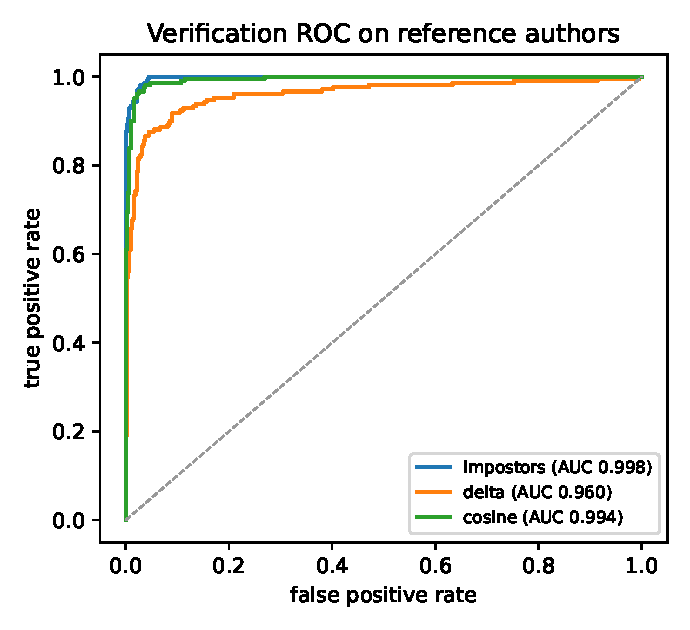
\includegraphics[width=0.72\linewidth]{figures/roc.pdf}
  \caption{Verification ROC on the reference authors for the three scorers. All lie well above chance; the impostors method is best.}
  \label{fig:roc}
\end{figure}

\paragraph{Calibration.} On held-out reference works the verifier separates same-author from different-author cases almost perfectly: genuine Severian works score a mean BDI of $0.86$ against Severian, other authors $0.09$ (AUC $\approx 1.0$; Figure~\ref{fig:calibration}). Scores are therefore interpretable on an absolute scale, and they are stable: across five random seeds the standard deviation of a group's score is $0.00$--$0.04$. Figure~\ref{fig:calibration} also shows that most pseudo-Chrysostom groups fall in the intermediate zone between the two reference distributions -- neither confidently Severian nor confidently foreign.

\begin{figure}[t]
  \centering
  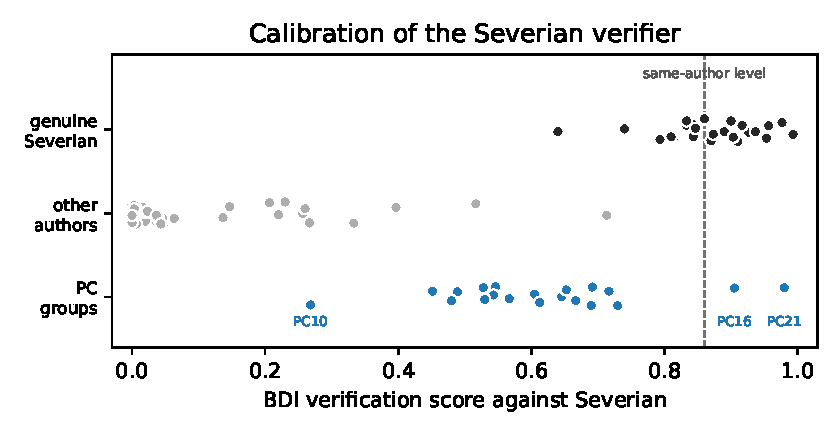
\includegraphics[width=0.92\linewidth]{figures/calibration.pdf}
  \caption{Calibration of the Severian verifier. Genuine Severian works (dark) and other authors (light) separate cleanly; the 22 PC groups (ticks) mostly sit between them.}
  \label{fig:calibration}
\end{figure}

\paragraph{The baseline over-attributes.} Nearest-centroid attribution assigns all 22 groups to Severian. This is an artifact: Severian is the largest homiletic author in the reference, so any homily drifts toward his centroid. The finding says little about authorship, and it disagrees with the scholarship (below).

\paragraph{Calibrated verdicts.} BDI is far more discriminating. Only two groups verify to Severian above the same-author level of $0.86$ -- PC21 ($0.98$) and PC16 ($0.90$); most sit in a consistent-but-unconfirmed band ($0.5$--$0.75$); and several point elsewhere. The full picture across the principal candidates is given in Figure~\ref{fig:heatmap}. The provenance control holds for 18 of 22 groups, and the four exceptions each prefer a different named author rather than a generic Patristic Text Archive profile.

\begin{figure}[t]
  \centering
  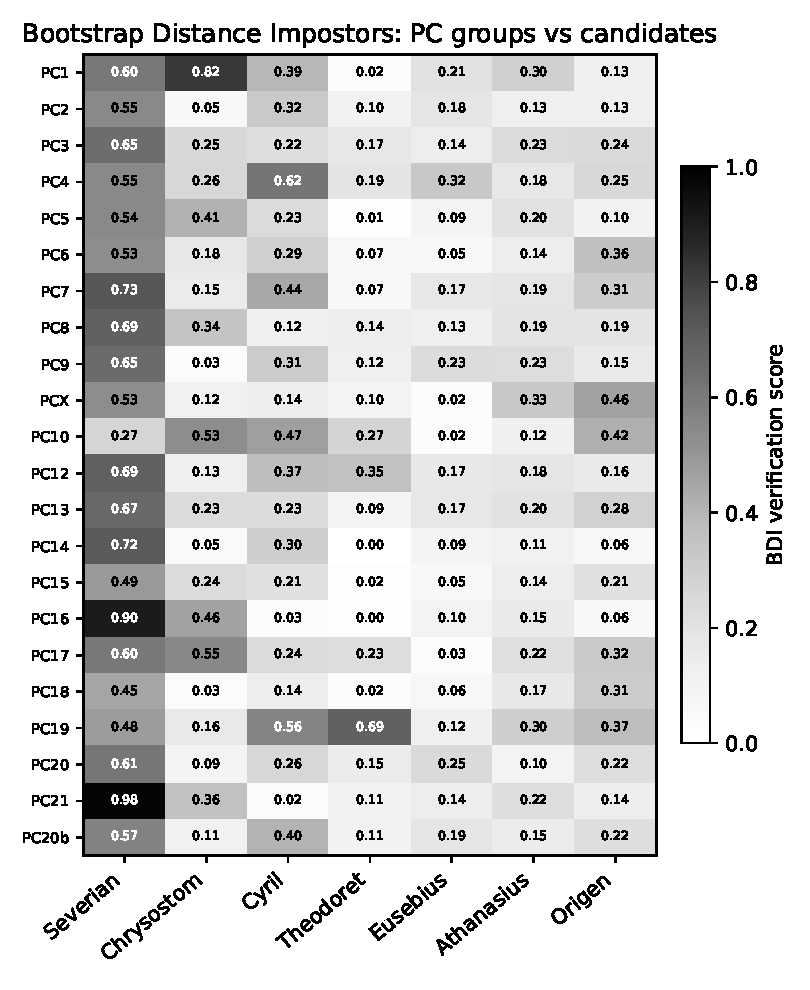
\includegraphics[width=\linewidth]{figures/heatmap.pdf}
  \caption{BDI verification score of each PC group against the principal candidate authors; darker is a stronger match. PC21 and PC16 verify to Severian, PC1 to Chrysostom, PC4 to Cyril, and PC19 to Theodoret.}
  \label{fig:heatmap}
\end{figure}

\subsection{A verifier that can abstain}

The verdicts so far are point estimates. Wrapping the impostors score in split-conformal prediction adds two things a philologist wants: an error guarantee and the option to answer ``not in this set of candidates.'' We check both on the reference. For held-out works whose author \emph{is} a candidate, the $90\%$ prediction set contains the true author $90\%$ of the time (mean size $1.12$) and the $80\%$ set $80\%$ of the time -- coverage is exact. For works whose author is \emph{not} a candidate, the set is empty $88\%$ of the time at $\alpha=0.10$ and $96\%$ at $\alpha=0.20$: the reject option fires when it should.

Applied to the pseudo-Chrysostoms at $\alpha=0.10$ (Table~\ref{tab:conformal}), the verifier returns a single author for thirteen of the twenty-two groups, an unresolved set for six, and abstains on three -- PC15, PC18, and the miscellany PCX, the same dispersed groups the internal-consistency check flags as possibly composite. Where scholarship names an author who is in the candidate set, the conformal set contains that author: PC9 and PC21 resolve to Severian alone, and PC1's set admits John Chrysostom.

The reject option is not, however, a remedy for an absent author who writes like a present one. The two ground-truth groups whose true author lies outside the candidate set are \emph{not} abstained: PC4 (Apollinaris) is absorbed by Cyril and PC12 (an Anomoean) by Severian, each as a confident singleton. Conformal coverage controls the \emph{average} rate at which absent authors slip through -- the $88$--$96\%$ measured above -- but it cannot flag an individual absent author who is a near stylistic neighbour of a candidate. This sharpens the closed-candidate boundary: the verifier knows when the author is, on average, out of the room, yet a sufficiently Cyril-like Apollinaris is still taken for Cyril.

\begin{table}[t]
  \centering
  \small
  % auto-generated by pc_conformal.py -- do not edit by hand
\begin{tabular}{lll}
\toprule
Group & $n$ & 90\% prediction set \\
\midrule
PC1 & 2 & Chrysostom, Severian \\
PC4 & 7 & Cyril \\
PC9 & 4 & Severian \\
PC12 & 2 & Severian \\
PC15 & 3 & \emph{abstains} \\
PC16 & 4 & Severian, Chrysostom \\
PC21 & 2 & Severian \\
\bottomrule
\end{tabular}

  \caption{Conformal $90\%$ prediction sets for selected pseudo-Chrysostom groups. PC9 and PC21 resolve to Severian and PC1 admits Chrysostom; PC15 abstains; PC4 and PC12 -- whose true authors (Apollinaris, an Anomoean) are absent from the candidate set -- are absorbed by a stylistic neighbour rather than abstained.}
  \label{tab:conformal}
\end{table}

\paragraph{Agreement with scholarship.} Five groups contain a work with a named modern attribution; these form a small ground-truth set (Table~\ref{tab:groundtruth}). Following \textcite{nagy2024}, we report each verdict as a statistical likelihood -- the fraction of the bootstrapped distance-difference distribution that favours the candidate -- with a 95\% confidence interval. For the three groups whose true author is one of our candidates the verifier is correct in every case: PC1 to Chrysostom, and PC21 and PC9 to Severian. Most striking is PC1, whose likelihood for Chrysostom ($0.85\,[0.83,0.86]$) exceeds that for Severian ($0.58\,[0.56,0.60]$) with non-overlapping intervals; PC1 is the one group scholarship regards as genuine Chrysostom (the \emph{In Genesim} sermons, \textsc{cpg} 4410), and the nearest-centroid baseline had wrongly placed it with Severian. The remaining two have true authors absent from the reference -- PC4 is assigned to Apollinaris, PC12 to a pair of Anomoean homilies \cite{liebaert1969} -- so the verifier cannot name them, though it correctly declines Chrysostom for both. Its errors are a limit of candidate coverage, not of discrimination.

\paragraph{Agreement with the neural verifier.} The reproduced Siamese network of \textcite{clerice2023}, trained on the same open data with the original settings (100 epochs, test AUC $0.91$) and scoring by its learned SNR-D distance, returns the same verdicts on the ground-truth groups: PC1 to Chrysostom, and PC21 and PC9 to Severian, together with the same PC12 miss. The interpretable impostors method and the neural metric-learner agree wherever the answer can be checked, so interpretability here costs no accuracy.

\paragraph{A frozen neural channel adds nothing.} A reviewer might still suspect that a modern contextual encoder would beat the hand-crafted features. It does not. Taking the Ancient-Greek BERT that produced our part-of-speech tags \cite{superpeitho} as a frozen document encoder -- inference only, no fine-tuning -- we mean-pool a $768$-dimensional embedding per text and treat it as a fourth verification channel. On the same $630$ benchmark problems it verifies authorship as accurately as the transparent features and no better (Table~\ref{tab:bert}): impostors on the neural embedding reach ROC-AUC $0.993$, against $0.995$ for the function-word, part-of-speech and affix channels combined. The two agree closely (Spearman $0.90$ across the benchmark), and on the pseudo-Chrysostoms they return the same leading candidate for nineteen of the twenty-two groups, including every ground-truth case -- PC1 to Chrysostom, PC9 and PC21 to Severian. Where they part (PC4, PC19) the neural channel leans to Severian, the corpus's dominant author, which is the pull calibration is meant to resist. A $768$-dimensional black box thus buys nothing over a thousand function words and some affixes, and it corroborates rather than overturns the interpretable verdicts.

\begin{table}[t]
  \centering
  \small
  % auto-generated by pc_bert.py -- do not edit by hand
\begin{tabular}{lccc}
\toprule
Channel & ROC-AUC & AP & $F_1$ \\
\midrule
Hand-crafted (FW+POS+AFF) impostors & 0.963 & 0.948 & 0.900 \\
BERT impostors & 0.946 & 0.926 & 0.888 \\
BERT cosine & 0.935 & 0.870 & 0.824 \\
\bottomrule
\end{tabular}

  \caption{A frozen Ancient-Greek BERT, used inference-only as a fourth channel, on the $630$-problem verification benchmark. Impostors on the neural embedding match the hand-crafted channels rather than improving on them.}
  \label{tab:bert}
\end{table}

\begin{table}[t]
  \centering
  \small
  \begin{tabular}{llccl}
\toprule
PC & CPG & SL$_{\text{Sev}}$ & SL$_{\text{Chry}}$ & Scholarship / check \\
\midrule
PC1 & 4410 & 0.58\,[0.56,0.60] & 0.85\,[0.83,0.86] & Chrysostom (genuine)~\checkmark \\
PC21 & 4564 & 0.97\,[0.97,0.98] & 0.35\,[0.34,0.38] & Severian (proposed)~\checkmark \\
PC9 & 4215 & 0.65\,[0.63,0.66] & 0.03\,[0.03,0.04] & contains Severian work~\checkmark \\
PC4 & 4606--12 & 0.55\,[0.54,0.56] & 0.26\,[0.25,0.27] & Apollinaris (absent)~(author absent) \\
PC12 & 2082/83 & 0.70\,[0.68,0.72] & 0.13\,[0.11,0.14] & Anomoean (absent)~(author absent) \\
\bottomrule
\end{tabular}

  \caption{Ground-truth groups. SL is the statistical likelihood (fraction of the bootstrapped distance-difference distribution favouring the candidate), with a 95\% bootstrap confidence interval. The verifier is correct for all three groups whose true author is a candidate (\checkmark); PC4 and PC12 have their true authors absent from the reference.}
  \label{tab:groundtruth}
\end{table}

\paragraph{Per-channel evidence.} The decomposition separates trustworthy verdicts from fragile ones (Table~\ref{tab:channels}). The confident Severian cases agree across all three channels: PC21 scores $0.85$/$0.86$/$0.95$ on function words, part-of-speech trigrams, and affixes. Among the divergent groups, PC19's lean toward Theodoret rests on function words ($0.71$), the channel least sensitive to orthography, and is the best-supported non-Severian proposal. By contrast the affix-driven leans -- PC1 toward Chrysostom ($\text{AFF}=0.91$) and PC4 toward Cyril ($\text{AFF}=0.67$), with part-of-speech evidence neutral or opposed -- must be read with caution, since character affixes may register editorial spelling as much as authorial habit.

\begin{table}[t]
  \centering
  \small
  \begin{tabular}{llccc}
    \toprule
    PC & Candidate & FW & POS & AFF \\
    \midrule
    PC21 & Severian   & 0.85 & 0.86 & 0.95 \\
    PC16 & Severian   & 0.77 & 0.67 & 0.90 \\
    PC19 & Theodoret  & 0.71 & 0.28 & 0.20 \\
    PC1  & Chrysostom & 0.62 & 0.44 & 0.91 \\
    PC4  & Cyril      & 0.48 & 0.07 & 0.67 \\
    \bottomrule
  \end{tabular}
  \caption{Per-channel BDI for selected groups. Confident verdicts (PC21, PC16) agree across channels; divergent ones are channel-dependent.}
  \label{tab:channels}
\end{table}

\paragraph{Proposals for the anonymous groups.} For the seventeen groups that scholarship leaves without an author, the verdicts are hypotheses rather than confirmations. Two are worth a philologist's attention: PC16 verifies to Severian at $0.90$ across all channels, and PC19 leans to Theodoret on function-word evidence. Each is offered with its full per-channel profile so that the basis of the proposal is open to inspection.

\subsection{Are the groups single authors?}

A group-level verdict presumes that each PC group is the work of one hand, yet the grouping is editorial and some clusters may be composite. We measure the internal cohesion of every multi-text group as the mean pairwise distance among its own texts, against a cross-group baseline of $0.81$ (Table~\ref{tab:internal} in the appendix). Most groups are markedly tighter than the baseline -- the seven sermons \emph{De ieiunio} (PC7) are the most cohesive at $0.28$, and PC16 at $0.41$ -- which supports reading them as authorial units. A few are as dispersed as random cross-group pairs: PC5, PC20, PC15, and PC3 sit near or above $0.85$. For those groups a single verification verdict may average over more than one author, and the prudent step is to verify their members individually.

\subsection{The stylometric neighbourhood}

The verification scores are corroborated by the unsupervised structure of the data. Figure~\ref{fig:dendrogram} clusters the PC group and candidate-author profiles under Burrows's Delta: Severian sits inside a branch of Severian-leaning groups (PC16, PC13, PC9, PC20, PC7), Chrysostom joins PC1, Theodoret joins PC10, and the dispersed groups PC5, PC12, PC19 and PCX fall out at the largest distances. A two-dimensional projection (Figure~\ref{fig:pca}) shows the same neighbourhoods, with PC1 beside Chrysostom and most groups gathered around the Antiochene authors; the low explained variance is expected for high-dimensional stylometric features and the clustering of Figure~\ref{fig:dendrogram} is the more reliable summary.

\begin{figure}[t]
  \centering
  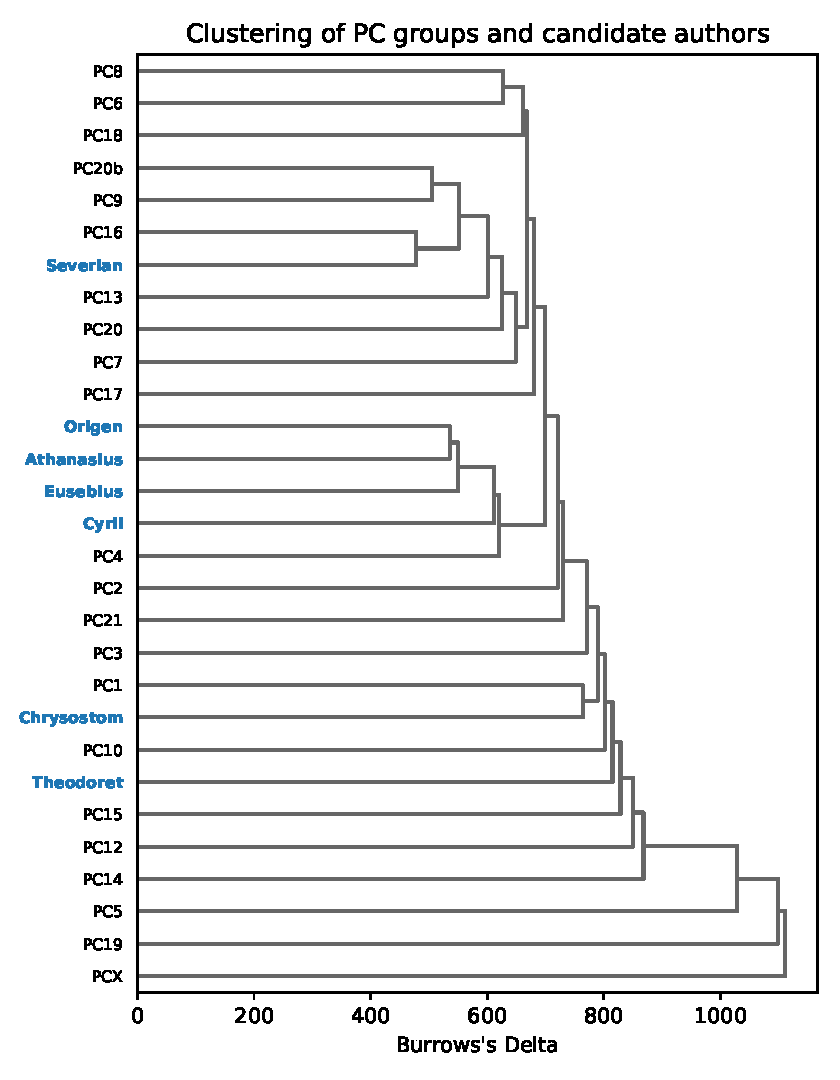
\includegraphics[width=0.96\linewidth]{figures/dendrogram.pdf}
  \caption{Hierarchical clustering (average linkage, Burrows's Delta) of the PC groups and candidate authors (authors in bold). PC1 clusters with Chrysostom; a Severian branch gathers PC16, PC13, PC9, PC20 and PC7.}
  \label{fig:dendrogram}
\end{figure}

\begin{figure}[t]
  \centering
  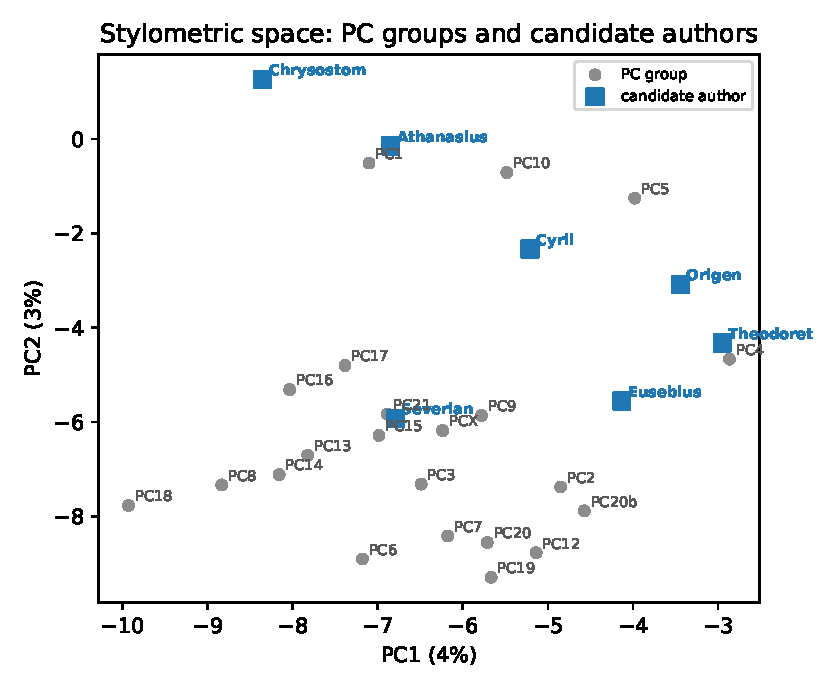
\includegraphics[width=0.96\linewidth]{figures/pca.pdf}
  \caption{Two-dimensional PCA projection (axes from the reference corpus) of PC groups (circles) and candidate authors (squares). PC1 sits beside Chrysostom.}
  \label{fig:pca}
\end{figure}

\subsection{Which words separate the rivals}

The verdicts rest on features a philologist can name. Table~\ref{tab:distinctive} lists the function words most distinctive of each rival, ranked by a Welch $t$-statistic over the reference-standardised frequencies. Severian's markers are narrative and citational -- \gk{λέγει} (``he says''), \gk{ἐγένετο} (``it came to pass''), \gk{ὅτε} (``when''), the movable-nu \gk{φησὶν} -- while Chrysostom's are the connectives of argument -- \gk{γάρ} (``for''), \gk{ἂν}, \gk{καθάπερ} (``just as''), \gk{οὐκέτι} (``no longer'') -- and the bare \gk{φησί}. The two even part company on a single orthographic reflex of the same verb of speaking, Severian preferring \gk{φησὶν} and Chrysostom \gk{φησί}. The part-of-speech channel agrees: Chrysostom is marked most strongly by adverb chains (the trigrams $d$--$d$--$v$ and $v$--$d$--$d$), Severian by nominal, narrative sequences.

These markers are not merely group-level averages; they track the individual verdicts. Projecting each group onto the Severian-minus-Chrysostom discriminator axis (positive leans Severian, negative Chrysostom) places the genuinely Chrysostomic PC1 on the Chrysostom side ($-0.065$) and the Severian-verified groups on the other (PC9 $+0.143$, PC21 $+0.126$, PC16 $+0.075$). The words that separate the two authors are the words that decide the attributions.

A last question is whether the historical confusion of the two men reflects a genuine likeness of style. It does not. A leave-one-out test separates their genuine works with $97\%$ accuracy over 35 homilies, and the distance between their centroids ranks only eleventh of twenty-one among candidate-author pairs -- no closer than Eusebius to Origen. The manuscripts merged the two because Severian preached in Chrysostom's city, in his genre and his lifetime, and his homilies travelled under the more famous name; their prose was never the reason. That the confusion is one of transmission and not of style is exactly what makes it tractable to a stylometric method.

\begin{table}[t]
  \centering
  \small
  % auto-generated by pc_distinctive.py -- do not edit by hand
\begin{tabular}{ll}
\toprule
Severian favours & John Chrysostom favours \\
\midrule
\gk{λέγει} & \gk{φησί} \\
\gk{τὴν} & \gk{τοῦτο} \\
\gk{ὁ} & \gk{ἂν} \\
\gk{ἐγένετο} & \gk{γάρ} \\
\gk{φησὶν} & \gk{τούτων} \\
\gk{ἡ} & \gk{εἶναι} \\
\gk{ὅτε} & \gk{καθάπερ} \\
\gk{ἐγὼ} & \gk{οὐκέτι} \\
\bottomrule
\end{tabular}

  \caption{Function words most distinctive of each rival, ranked by a Welch $t$-statistic over reference-standardised frequencies. Severian favours narrative and citational words; Chrysostom favours the connectives of argument.}
  \label{tab:distinctive}
\end{table}

\section{Discussion}

The exercise carries a methodological lesson beyond the individual verdicts. A nearest-neighbour reading of an imbalanced reference manufactures a consensus -- here, ``everything is Severian'' -- that neither calibration nor the scholarship supports. Calibrated verification with an explicit impostor set, a provenance control, and a per-channel breakdown recovers a defensible and inspectable picture: it reproduces named attributions where they exist, including the sole genuine Chrysostom, and it declines to over-commit on the rest. That the interpretable representation is no sacrifice of accuracy is worth stating plainly: both a trained Siamese metric and a frozen contextual encoder, added as extra channels, match the hand-crafted features without beating them and agree with their verdicts -- legibility here is free.

\paragraph{Limitations.} The reference, though open, is a single assemblage; author families it lacks (the Anomoean PC12) cannot be found, and this is a boundary of any closed-candidate method. Affix-driven verdicts may reflect orthographic normalisation in the editions rather than authorship, a caveat the per-channel view makes visible but does not remove. The two Severian-positive ground-truth attributions (PC9's \textsc{cpg} 4215; PC21's \textsc{cpg} 4564) rest on the current editorial consensus, itself in part still argued; our agreement corroborates but does not settle them. Finally, the proposals for the anonymous groups are starting points for philological work, not conclusions.

\section{Conclusion}

Interpretable, feature-based stylometry remains a serviceable instrument for disputed patristic authorship when it is equipped to make -- and to explain -- a verification claim, and to decline one. On open Greek data, an open-set conformal protocol reproduces the published attribution of the pseudo-Chrysostoms where scholarship provides one, identifies the single genuinely Chrysostomic group without prompting, offers confidence-graded, per-channel proposals for the anonymous remainder, and -- with a distribution-free guarantee -- abstains when the author is not among the candidates. That neither a retrained Siamese nor a frozen encoder improves on the hand-crafted features shows that this legibility costs nothing in accuracy. The result is not a black box that pronounces, but an instrument a philologist can interrogate -- and one that says when it cannot answer.

\printbibliography

\appendix

\section{Full results}

Table~\ref{tab:full} reports every PC group with its \textsc{cpg} number, its BDI score against Severian and against Chrysostom, and the current scholarly attribution. Table~\ref{tab:internal} reports the internal cohesion of the multi-text groups.

\begin{table}[h]
  \centering
  \small
  \begin{tabular}{llccl}
\toprule
PC & CPG & BDI$_{\text{Sev}}$ & BDI$_{\text{Chry}}$ & Scholarship \\
\midrule
PC1 & 4410 & 0.61 & 0.84 & John Chrysostom (genuine) \\
PC2 & 4566/4567 & 0.55 & 0.06 & anonymous ps.-Chrysostom \\
PC3 & 4579/4580/4641 & 0.65 & 0.25 & anonymous ps.-Chrysostom \\
PC4 & 4606-4612 & 0.53 & 0.27 & Apollinaris of Laodicea (serm.1-3) \\
PC5 & 4603 & 0.53 & 0.38 & anonymous ps.-Chrysostom \\
PC6 & 4615-4617 & 0.55 & 0.18 & anonymous ps.-Chrysostom \\
PC7 & 4619 & 0.72 & 0.16 & anonymous ps.-Chrysostom \\
PC8 & 4620/4621 & 0.68 & 0.36 & anonymous ps.-Chrysostom \\
PC9 & 4215+4657/4659/4660 & 0.65 & 0.03 & MIXED: Severian (4215, firm) + Cap \\
PCX & 4667? & 0.55 & 0.14 & anonymous ps.-Chrysostom \\
PC10 & 4516 & 0.28 & 0.56 & anonymous ps.-Chrysostom \\
PC12 & 2082/2083 & 0.71 & 0.16 & Anomoean/Neo-Arian (Liebaert) - NO \\
PC13 & 4506/4525/epiph. & 0.66 & 0.25 & anon; epiphany hom. 'Severian?' (W \\
PC14 & 4618 & 0.72 & 0.04 & anonymous ps.-Chrysostom \\
PC15 & 4589/4669/4969 & 0.45 & 0.24 & anonymous ps.-Chrysostom \\
PC16 & 4701/4576/4544/4545 & 0.90 & 0.45 & anonymous ps.-Chrysostom \\
PC17 & 4626/4585 & 0.58 & 0.54 & anonymous ps.-Chrysostom \\
PC18 & 4587/4577 & 0.45 & 0.05 & anonymous ps.-Chrysostom \\
PC19 & 4601 & 0.51 & 0.17 & anonymous ps.-Chrysostom \\
PC20 & 4631/4547/4757/4571/4658 & 0.60 & 0.10 & anonymous ps.-Chrysostom \\
PC21 & 4564 & 0.98 & 0.38 & Severian of Gabala (proposed) \\
PC20b & 4629/4588/4699+ & 0.57 & 0.13 & MIXED: Cappadocian (3) + anon \\
\bottomrule
\end{tabular}

  \caption{All 22 pseudo-Chrysostom groups: CPG number, BDI scores against Severian and Chrysostom, and current scholarly attribution.}
  \label{tab:full}
\end{table}

\begin{table}[h]
  \centering
  \small
  \begin{tabular}{lcc}
\toprule
PC & \#texts & mean within-group dist. \\
\midrule
PC7 & 7 & 0.278 \\
PC16 & 4 & 0.411 \\
PC18 & 2 & 0.542 \\
PC10 & 2 & 0.561 \\
PC21 & 2 & 0.592 \\
PC1 & 2 & 0.612 \\
PC2 & 2 & 0.623 \\
PC17 & 2 & 0.638 \\
PC12 & 2 & 0.696 \\
PC4 & 7 & 0.708 \\
PC6 & 3 & 0.710 \\
PC8 & 2 & 0.775 \\
PC13 & 3 & 0.791 \\
PC9 & 4 & 0.817 \\
PC20b & 9 & 0.843 \\
PC3 & 3 & 0.846 \\
PC15 & 3 & 0.853 \\
PC20 & 5 & 0.853 \\
PC5 & 2 & 0.878 \\
\midrule
cross-group baseline & -- & 0.810 \\
\bottomrule
\end{tabular}

  \caption{Internal cohesion of the multi-text PC groups: mean pairwise distance among a group's own texts (lower is tighter). The cross-group baseline is $0.81$.}
  \label{tab:internal}
\end{table}

\end{document}
